\documentclass[journal,comsoc]{IEEEtran}
\usepackage[T1]{fontenc}% optional T1 font encoding

\usepackage{ifpdf}
\usepackage{cite}
\ifCLASSINFOpdf
  \usepackage[pdftex]{graphicx}
\else
  \usepackage[dvips]{graphicx}
\fi
\usepackage{amsmath}
\interdisplaylinepenalty=2500
\usepackage[cmintegrals]{newtxmath}
\usepackage{bm}
\usepackage{algorithmic}
\usepackage{array}
\ifCLASSOPTIONcompsoc
  \usepackage[caption=false,font=normalsize,labelfont=sf,textfont=sf]{subfig}
\else
  \usepackage[caption=false,font=footnotesize]{subfig}
\fi
%\usepackage{fixltx2e}
%\usepackage{stfloats}
\ifCLASSOPTIONcaptionsoff
  \usepackage[nomarkers]{endfloat}
 \let\MYoriglatexcaption\caption
 \renewcommand{\caption}[2][\relax]{\MYoriglatexcaption[#2]{#2}}
\fi
\usepackage{url}
\usepackage{hyperref}
% correct bad hyphenation here
\hyphenation{op-tical net-works semi-conduc-tor}


\begin{document}
\title{Temporal-Spatial Depth Map Based Hand Pose Estimation}

\author{{Anonymous}% <-this % stops a space
\thanks{Anonymous}}

% The paper headers
\markboth{Journal of \LaTeX\ Class Files,~Vol.~14, No.~8, August~2015}%
{Shell \MakeLowercase{\textit{et al.}}: Bare Demo of IEEEtran.cls for IEEE Communications Society Journals}

% make the title area
\maketitle

\begin{abstract}
Abstract
\end{abstract}

% Note that keywords are not normally used for peerreview papers.
\begin{IEEEkeywords}
Hand pose estimation, LSTM, mixture of experts.
\end{IEEEkeywords}


% For peer review papers, you can put extra information on the cover
% page as needed:
\ifCLASSOPTIONpeerreview
\begin{center} \bfseries EDICS Category: 3-BBND \end{center}
\fi
%
% For peerreview papers, this IEEEtran command inserts a page break and
% creates the second title. It will be ignored for other modes.
\IEEEpeerreviewmaketitle



\section{Introduction}\label{sec:introduction}
\IEEEPARstart{H}{and} pose estimation plays an pivotal role in application of human-computer interface(HCI) and augmentation reality(AR).
So far, there are a plenty of researches on this topic\cite{guo2017region}, but it is still challenge to estimate hand pose in the actual scene
owing to the large view variance, high joint flexibility, poor depth quality, severe self-occlusion and similar part confusion.

We summary our contribution in the following two folds:
\begin{itemize}
  \item
  We integrate features from depth map and 3D volumetric representation for hand pose estimation.
  The experiment reveals that 3D volumetric representation helps the hand structure.
  \item
  To our knowledge, it is the first time to consider temporal context in hand pose estimation.
  We model the coherence among frames by LSTM, and implement a hand pose estimation system with an eye to accuracy,
  efficiency, robustness and stability simultaneously.
  \item
  We evaluate our approach on two open datasets( e.g. NYU and ICVL), and get the comparable results.
\end{itemize}

% needed in second column of first page if using \IEEEpubid
%\IEEEpubidadjcol

%-------------------------------------------------------------------------
\section{Related Work}\label{sec:related work}
\subsection{Hand Pose Estimation}
\subsection{Mixture of Experts}
\subsection{LSTM}


%------------------------------------------------------------------------
\section{Our Method}\label{sec:our method}
% prepare the notation for problem
Our objective is to predict the 3D hand joint locations from a depth image, the locations are represented as a set of keypoints.
We give some notations about the problem. We denote a sequence of depth images as $\mathcal{I}=\{I_t\}_{t=1}^T$,
and the corresponding hand poses are $\mathcal{P}=\{P_t\}_{t=1}^T$. $P_t$ is the pose of hand in the form of $n$
hand joints of its joints $P_t=\{j_i\}_i^n$ with $j_i=(x_i,y_i,z_i)$ from the depth image $I_t$.

In the following, we describe our proposed method for hand pose estimation. Figure~\ref{fig:architecture} shows the entire
architecture. Aspired by Mixture of Experts~\cite{jacobs1991adaptive}, we use a gating network to
control two expert networks. In general, network is composed of two parts: gating network and expert networks.
Each experts predicts the 3D pose given the input, gating network weights the prediction by each experts.
The experts concentrate on different information. LSTM-CNN takes temporal context into account between the consecutive frames.
Fusion-CNN, thinking over spatial information, fuses the features from depth map and 3D volumetric representation.
The LSTM-CNN and Fusion-CNN we employ are discussed in Section~\ref{sec:lstm netowork} and Section~\ref{sec:fusion network}.
And the mixture of experts are discussed in Section~\ref{sec:gating network}.

\begin{figure}[t]
    \centering
    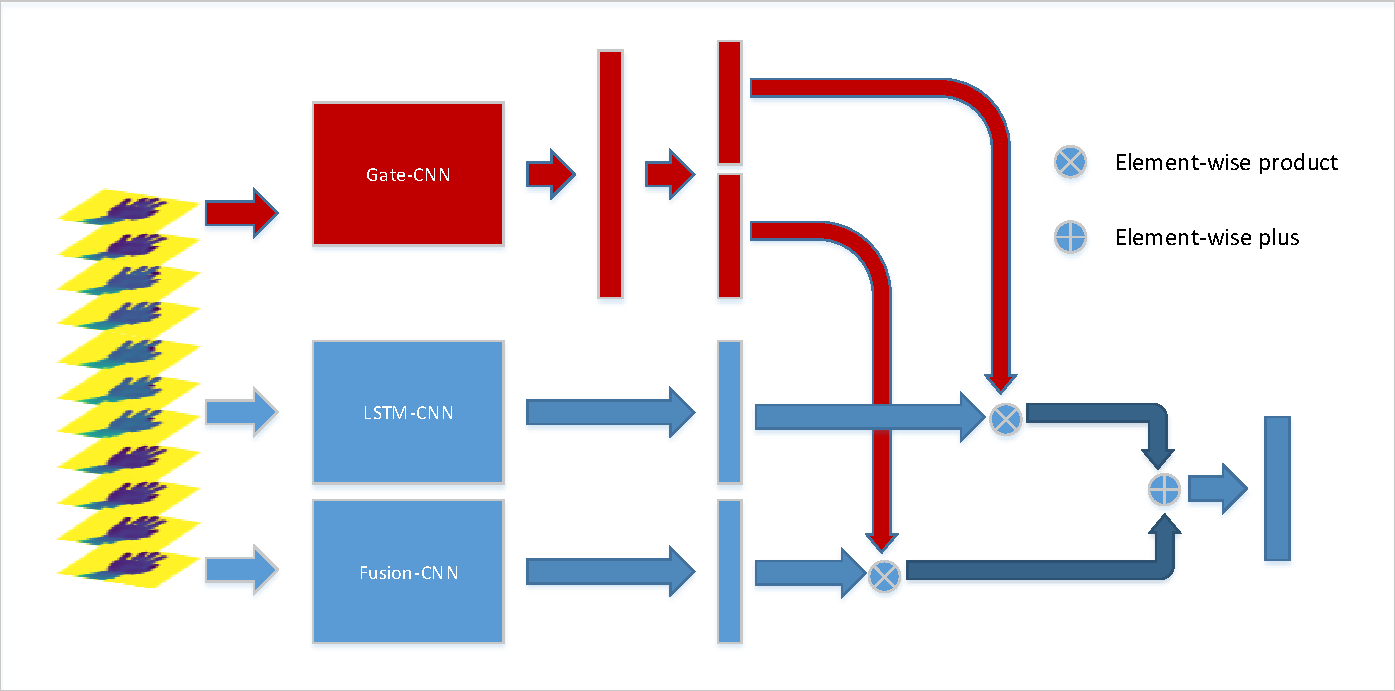
\includegraphics[width=1\linewidth]{src/network/architecture.pdf}
    \caption{The overview of architecture. The red branch is the gating network, the blue branch is the expert networks.
    Each expert predicts the 3D pose given the input, gating network weights the prediction by each experts.}
\label{fig:architecture}
\end{figure}

\subsection{LSTM Based Network}\label{sec:lstm netowork}
As we know, the hand poses between successive frames are correlated (e.g. when grabbing, the joints on fingers are most likely
to be closer). However, there are still no approaches considering the coherence of successive frames in hand pose estimation.

Currently, an Recurrent Neural Network(RNN) with Long Short-Term Memory(LSTM) units~\cite{zaremba2014learning} is widely used
because they are expressive and easy to train. The LSTM network is mostly used for modeling the long term temporal correspondence.
As the architecture in Fig~\ref{fig:lstm network}, the input is a sequence of frames $\{I_1, I_2, \dots, I_N\}$.
Based on a simple baseline network shown in Fig~\ref{fig:baseline network}, we replace the last fully connected layer with an LSTM.
To reserve the original features, we concatenate features from first fully connected layer and LSTM, and regress hand joint locations.


\begin{figure*}[t]
    \centering
    \subfloat[Baseline Network.]{
        \label{fig:baseline network}
        \begin{minipage}[t]{240pt}
            \centering
            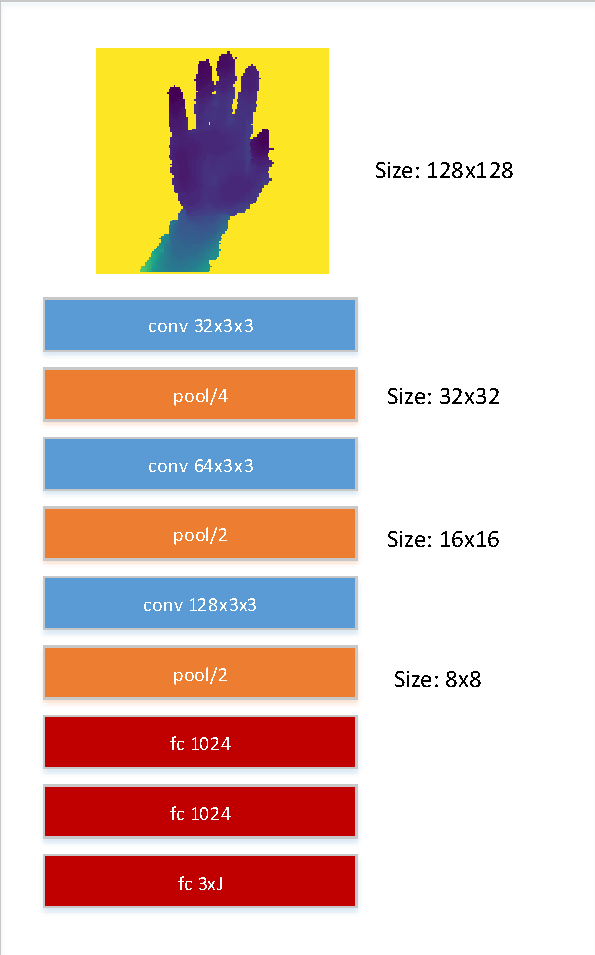
\includegraphics[width=0.805\linewidth]{src/network/baseline.pdf}
        \end{minipage}
    }
    \subfloat[LSTM CNN.]{
        \label{fig:lstm network}
        \begin{minipage}[t]{240pt}
            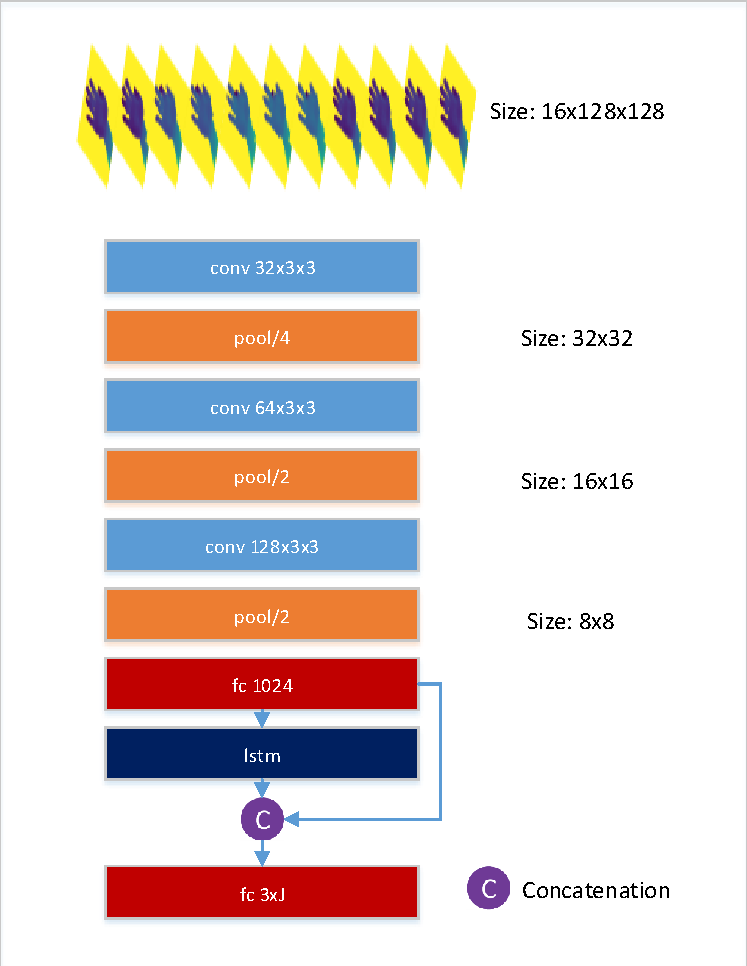
\includegraphics[width=1\linewidth]{src/network/lstm.pdf}
        \end{minipage}
    }
\caption{Baseline and LSTM-CNN network. Regressing the hand joint location in 3D.}
\label{fig:baseline and lstm network}
\end{figure*}


\subsection{Fusion Network}\label{sec:fusion network}
According to the discussion in \cite{supancic2015depth} and \cite{deng2017hand3d}, 3D volumetric representation helps the hand
pose estimation. So we project the hand in 2D depth map into 3D space, a bit difference is we slice the space into 8 layers to
preserve details, as shown in Fig.~\ref{fig:fusion network}. The 3D volumetric representation keep the structure of hand, we
can clearly find all finger tips in the first layer.

In our opinion, the 3D volumetric representation is easier for constructing the hand structure, but it makes harder to estimate
the depth of hand joints. To obtain the structure information and depth information simultaneously, we combine these two kinds
of representation together. In Fig.~\ref{fig:fusion network}, we deploy a Deep-Fusion framework~\cite{chen2016multi} to fuse
the features. In the fusion network, the different features are fused together hierarchically. which could be expressed as:
\begin{equation}\label{eq:deep fusion}
\begin{aligned}
&f_0 = f_{depth} \oplus f_{3D} \\
&f_l = \textbf{H}_l^{depth}(f_{l-1}) \oplus \textbf{H}_l^{3D}(f_{l-1}) \\
&\forall l=1, \dots , L
\end{aligned}
\end{equation}
The $\oplus$ is element-wise mean, $\textbf{H}$ is the transformation for features, $l$ is the index for layer.

What's more, to obtain a robust feature, we use an auxiliary loss as the regularization. In Fig.~\ref{fig:fusion network},
the auxiliary path is useful only in training phase, and the layers connected by the blue dotted line share weights.
When training, the total losses are composed by three losses, i.e. three regression loss in different branches.
When testing, the auxiliary pathes are removed.
\begin{figure*}[t]
    \centering
    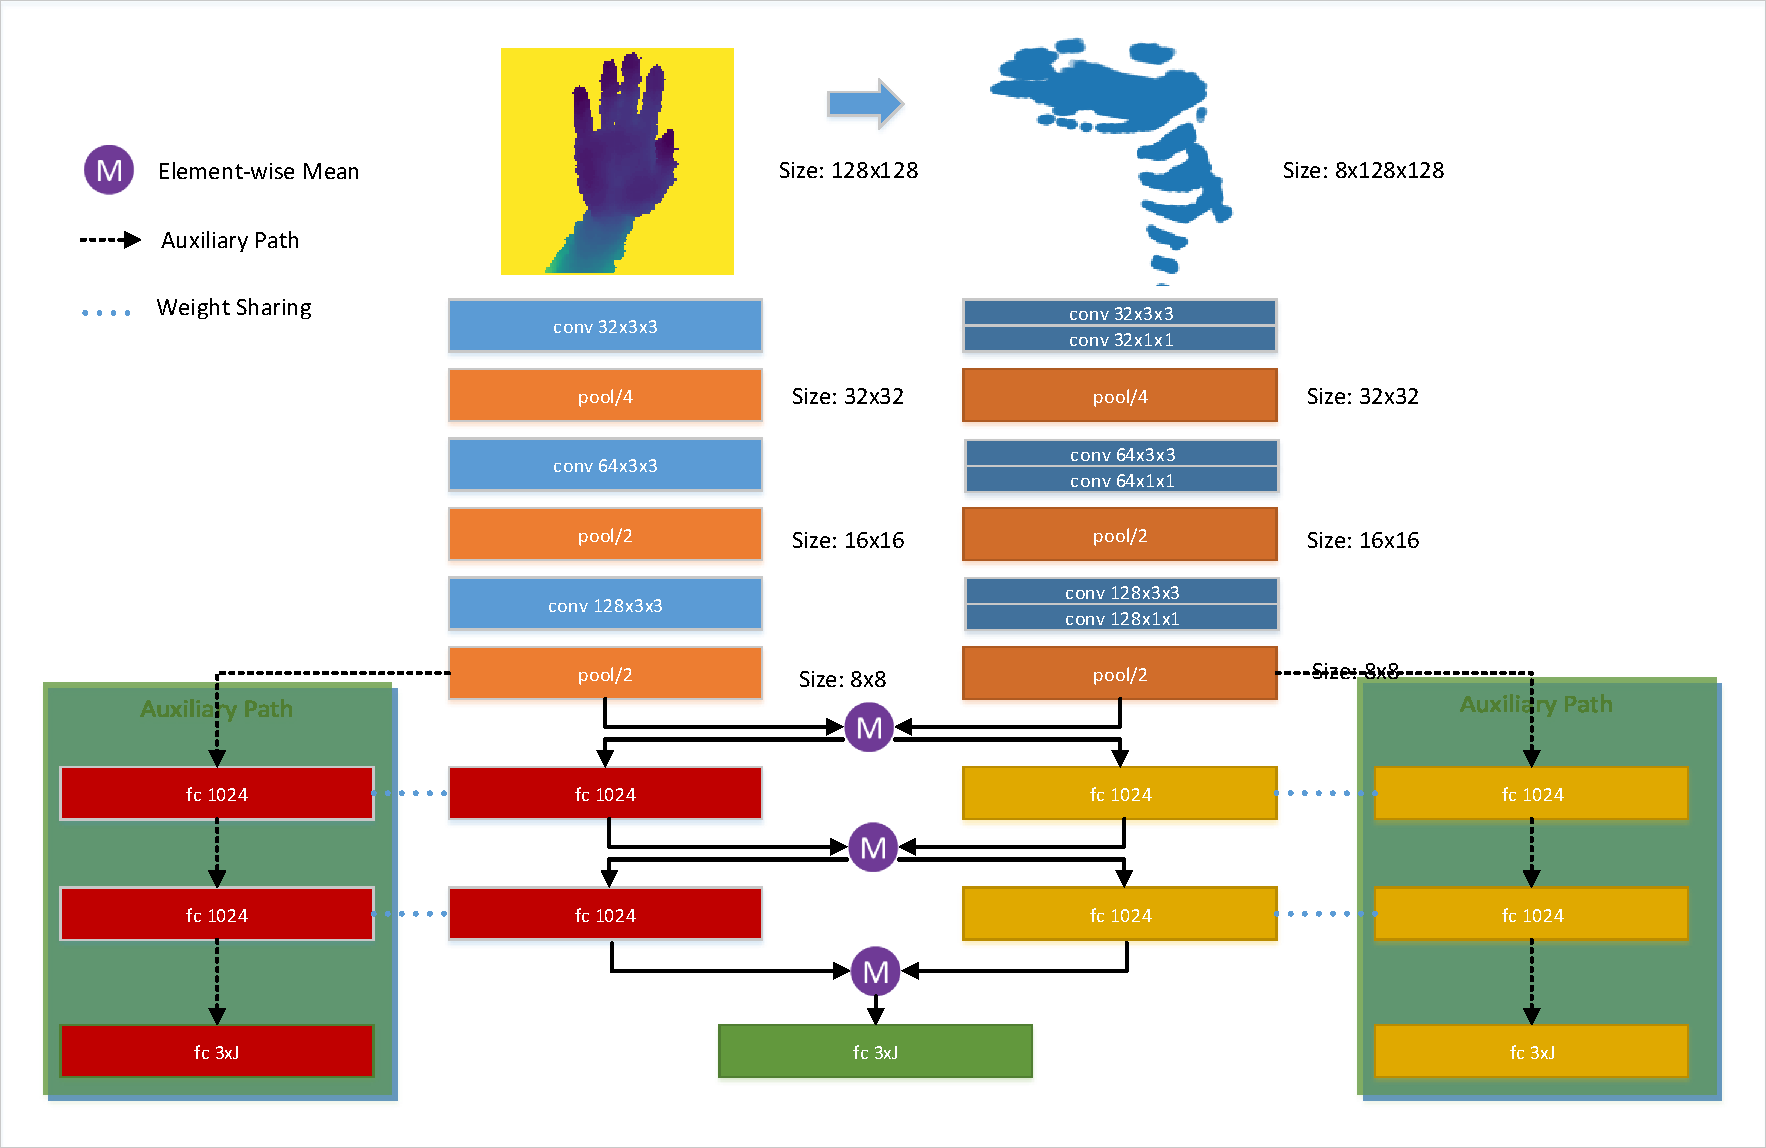
\includegraphics[width=1\linewidth]{src/network/fusion.pdf}
    \caption{Fusion Network}
\label{fig:fusion network}
\end{figure*}

\subsection{Gating Network}\label{sec:gating network}
With two networks stand in the different view for estimating the joints, we want to ensemble their advantages for last prediction.
Jacob. et al proposed Mixture of Experts(MoE)~\cite{jacobs1991adaptive} for adaptively integrating different regressors.

Gating network weights two predictors, and give out the last prediction according to the weights of predictions as follow:
\begin{equation}\label{eq:gating network}
\centering
\textbf{y} = \sum_{k=1}^K \textbf{g}_k \textbf{e}_k
\end{equation}
where $K$ is the number of experts, and $\textbf{e}_k$ is the output of $k$-th expert, $\textbf{g}_k$ is the $k$-th weight value of
gating network. The prediction $\textbf{y}$ is estimated as the weighted sum of each output $\textbf{e}_k$.

Because LSTM-CNN network considers the temporal information and Fusion network extracts the spatial information, mixture of experts
infer the hand joint location based on spatial-temporal features. Generally, gating network weights two predictions, it is more difficult
than prediction job. Thus, we double the parameters in the gating network than the base network, and employ Dropout~\cite{srivastava2014dropout}
after the fully connected layer to prevent overfitting.


%\begin{figure}[t]
%    \centering
%    \includegraphics[width=1\linewidth]{}
%    \caption{Gating Network}
%\label{fig:gating network}
%\end{figure}


%-------------------------------------------------------------------------
\section{Experiments}\label{sec:experiments}
In this section, we evaluate our approach on two public datasets, NYU~\cite{tompson2014real} and ICVL~\cite{tang2014latent}, for comparison
with the state-of-art methods. NYU dataset is composed of 72,757 training and 8,252 testing images, the resolution is 640x480. The dataset
is captured by PrimeSense, and the annotation is obtained by model-based tracking with a Particle Swarm Optimization processing. This dataset
is challenge because of its wider pose variation and noisy image yet some incorrect annotations. ICVL dataset is smaller than NYU dataset, contains
22,061 frames for training and 1,596 frames for testing. The resolution of images is 320x240 and captured by Creative Interactive Gesture Camera. The scale
of image is small and the annotation accuracy is limited, these makes the estimation hard.

The evaluation follows the standard metrics proposed in~\cite{tompson2014real}, including a plot of the percentage of test samples given a maximum
distance from ground truth and average distance error (in mm). There are totally 36 annotated joints in NYU dataset, but we only evaluate a subset of 14 joints
for a fair comparison with~\cite{tompson2014real,oberweger2015hands,oberweger2015training}. In addition to ICVL dataset, we evaluate 16 annotated joints for
comparison.
\subsection{Implementation Details}\label{sec:implementation}
We implement the training and testing using Caffe\cite{jia2014caffe}. The segmentation step follows~\cite{oberweger2015hands} to extract a cube from the depth image,
and the cube is resized to a 128x128 depth image with the depth value normalized to [-1, 1]. Moreover, we augment the dataset by random rotation.

The three parts of network are trained separately. The baseline network is pre-trained for LSTM-CNN and Fusion network using Adam, we set the learning rate as 1e-3
and train the network for 100,000 iterations, the learning rate is divided by 10 every 20,000 iterations and the mini-batch is set as 128. LSTM-CNN and Fusion network
trained based on the baseline network with the parameters fixed, and the configuration is same except that we only train the network for 50,000 iterations. To train
Gating network, the parameters are all fixed but the parameters in gate branch and the network is trained for 50,000 iterations. Our training takes place on machines
equipped with a 12GB Titan X GPU and 64GB memory.
\subsection{Comparison with State-of-art}\label{sec:comparison}
We compare our approach with several CNN based hand pose estimation method. We compare with four methods~\cite{tompson2014real}\cite{oberweger2015hands}
\cite{oberweger2015training}\cite{zhou2016model} on NYU dataset, and compare with two methods~\cite{oberweger2015hands}\cite{zhou2016model} on ICVL dataset.
The mean error of different methods is shown in Tab.~\ref{tab:mean error NYU} and Tab.~\ref{tab:mean error ICVL} as well as average error shown in Fig.~\ref{fig:Qualitative result NYU}.

\begin{table}[htbp]\footnotesize
\centering
    \begin{tabular}{|c|c|c|c|c|c|}
    \hline
    Methods        &\cite{tompson2014real} &\cite{oberweger2015hands} &\cite{oberweger2015training} &\cite{zhou2016model} &Ours\\
    \hline
    Mean Error(mm) &21.0                   &20.8                      &15.9                         &16.9                 &14.8\\
    \hline
\end{tabular}
\vspace{1em}
\caption{Comparison between our approach and state-of-art methods for mean error.}
\label{tab:mean error NYU}
\end{table}

\begin{table}[htbp]\footnotesize
\centering
    \begin{tabular}{|c|c|c|c|}
    \hline
    Methods        &\cite{oberweger2015hands} &\cite{zhou2016model} &Ours\\
    \hline
    Mean Error(mm) &0                      &0                       &0\\
    \hline
    \end{tabular}
\vspace{1em}
\caption{Comparison between our approach and state-of-art methods for mean error.}
\label{tab:mean error ICVL}
\end{table}

\begin{figure*}[t]\footnotesize
\centering
    \subfloat[]{
        \label{fig:comparison NYU}
        \begin{minipage}[t]{200pt}
            \centering
            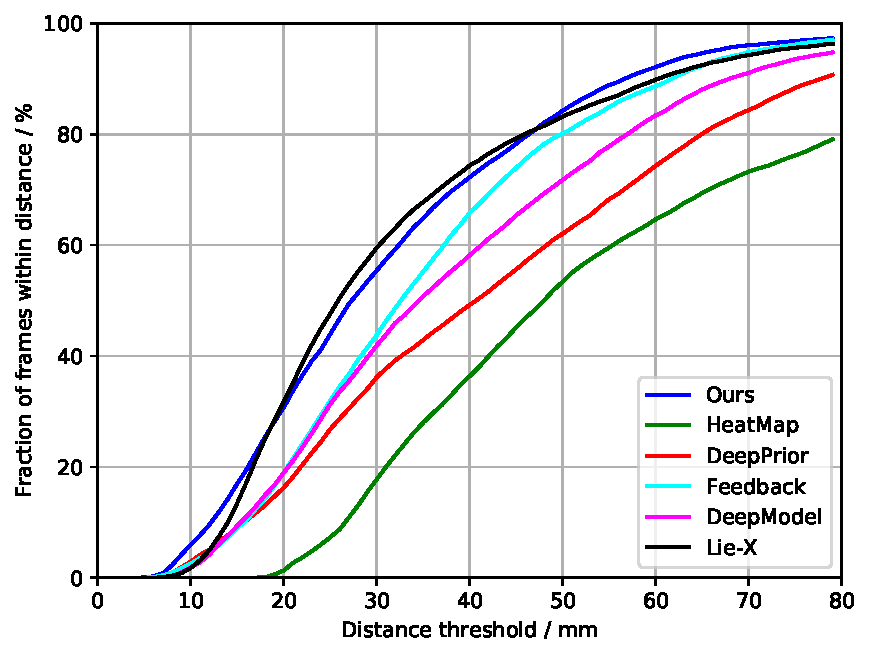
\includegraphics[width=1\linewidth]{src/experiment/eval/NYU_comparison/comparison_frameswithin.pdf}
        \end{minipage}
    }
    \subfloat[]{
        \label{fig:joint mean NYU}
        \begin{minipage}[t]{260pt}
            \centering
            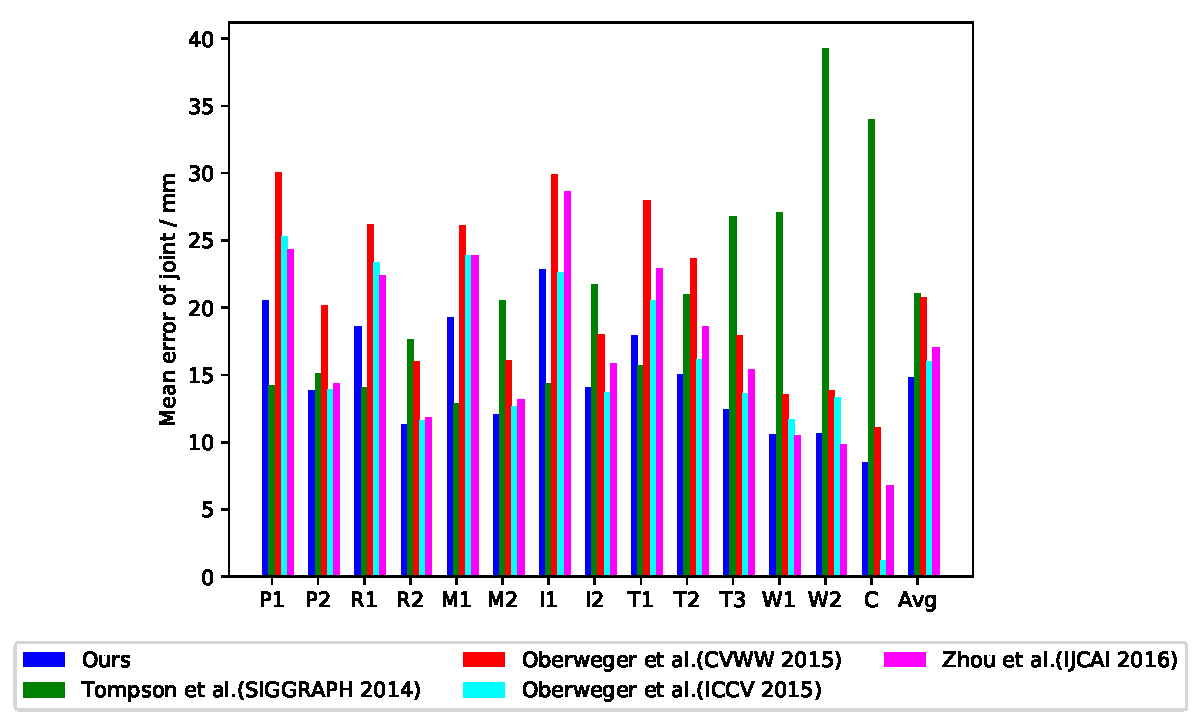
\includegraphics[width=1\linewidth]{src/experiment/eval/NYU_comparison/comparison_joint_mean.pdf}
        \end{minipage}
    }
    \caption{Qualitative results for NYU dataset.}
    \label{fig:Qualitative result NYU}
\end{figure*}
\subsection{Ablation}\label{sec:ablation}
To show the effects of different parts in mixed network, we do the ablation experiments. We show the test result on NYU and ICVL dataset in Fig.~\ref{fig:Qualitative result ablation}.

\begin{figure*}[t]\footnotesize
\centering
    \subfloat[]{
        \label{fig:ablation NYU}
        \begin{minipage}[t]{200pt}
            \centering
            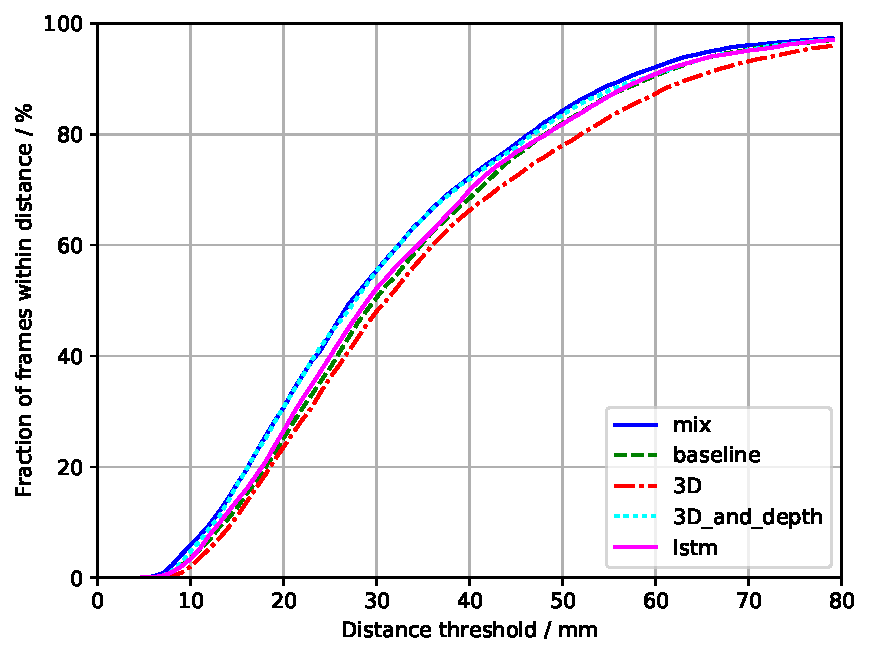
\includegraphics[width=1\linewidth]{src/experiment/eval/NYU_ablation/ablation_frameswithin.pdf}
        \end{minipage}
    }
    \subfloat[]{
        \label{fig:ablation joint mean NYU}
        \begin{minipage}[t]{180pt}
            \centering
            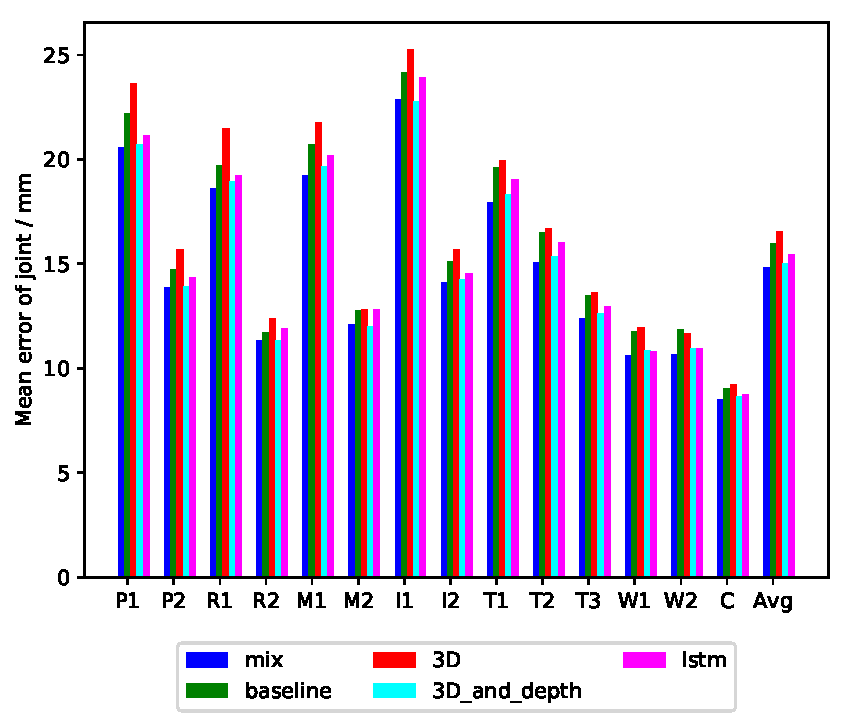
\includegraphics[width=1\linewidth]{src/experiment/eval/NYU_ablation/ablation_joint_mean.pdf}
        \end{minipage}
    }
    \caption{Qualitative results for ablation experiments.}
    \label{fig:Qualitative result ablation}
\end{figure*}

\section{Conclusion}\label{sec:conclusion}
The conclusion goes here.

% An example of a floating figure using the graphicx package.
% Note that \label must occur AFTER (or within) \caption.
% For figures, \caption should occur after the \includegraphics.
% Note that IEEEtran v1.7 and later has special internal code that
% is designed to preserve the operation of \label within \caption
% even when the captionsoff option is in effect. However, because
% of issues like this, it may be the safest practice to put all your
% \label just after \caption rather than within \caption{}.
%
% Reminder: the "draftcls" or "draftclsnofoot", not "draft", class
% option should be used if it is desired that the figures are to be
% displayed while in draft mode.
%
%\begin{figure}[!t]
%\centering
%\includegraphics[width=2.5in]{myfigure}
% where an .eps filename suffix will be assumed under latex,
% and a .pdf suffix will be assumed for pdflatex; or what has been declared
% via \DeclareGraphicsExtensions.
%\caption{Simulation results for the network.}
%\label{fig_sim}
%\end{figure}

% Note that the IEEE typically puts floats only at the top, even when this
% results in a large percentage of a column being occupied by floats.


% An example of a double column floating figure using two subfigures.
% (The subfig.sty package must be loaded for this to work.)
% The subfigure \label commands are set within each subfloat command,
% and the \label for the overall figure must come after \caption.
% \hfil is used as a separator to get equal spacing.
% Watch out that the combined width of all the subfigures on a
% line do not exceed the text width or a line break will occur.
%
%\begin{figure*}[!t]
%\centering
%\subfloat[Case I]{\includegraphics[width=2.5in]{box}%
%\label{fig_first_case}}
%\hfil
%\subfloat[Case II]{\includegraphics[width=2.5in]{box}%
%\label{fig_second_case}}
%\caption{Simulation results for the network.}
%\label{fig_sim}
%\end{figure*}
%
% Note that often IEEE papers with subfigures do not employ subfigure
% captions (using the optional argument to \subfloat[]), but instead will
% reference/describe all of them (a), (b), etc., within the main caption.
% Be aware that for subfig.sty to generate the (a), (b), etc., subfigure
% labels, the optional argument to \subfloat must be present. If a
% subcaption is not desired, just leave its contents blank,
% e.g., \subfloat[].


% An example of a floating table. Note that, for IEEE style tables, the
% \caption command should come BEFORE the table and, given that table
% captions serve much like titles, are usually capitalized except for words
% such as a, an, and, as, at, but, by, for, in, nor, of, on, or, the, to
% and up, which are usually not capitalized unless they are the first or
% last word of the caption. Table text will default to \footnotesize as
% the IEEE normally uses this smaller font for tables.
% The \label must come after \caption as always.
%
%\begin{table}[!t]
%% increase table row spacing, adjust to taste
%\renewcommand{\arraystretch}{1.3}
% if using array.sty, it might be a good idea to tweak the value of
% \extrarowheight as needed to properly center the text within the cells
%\caption{An Example of a Table}
%\label{table_example}
%\centering
%% Some packages, such as MDW tools, offer better commands for making tables
%% than the plain LaTeX2e tabular which is used here.
%\begin{tabular}{|c||c|}
%\hline
%One & Two\\
%\hline
%Three & Four\\
%\hline
%\end{tabular}
%\end{table}


% Note that the IEEE does not put floats in the very first column
% - or typically anywhere on the first page for that matter. Also,
% in-text middle ("here") positioning is typically not used, but it
% is allowed and encouraged for Computer Society conferences (but
% not Computer Society journals). Most IEEE journals/conferences use
% top floats exclusively.
% Note that, LaTeX2e, unlike IEEE journals/conferences, places
% footnotes above bottom floats. This can be corrected via the
% \fnbelowfloat command of the stfloats package.

% if have a single appendix:
%\appendix[Proof of the Zonklar Equations]
% or
%\appendix  % for no appendix heading
% do not use \section anymore after \appendix, only \section*
% is possibly needed

% use appendices with more than one appendix
% then use \section to start each appendix
% you must declare a \section before using any
% \subsection or using \label (\appendices by itself
% starts a section numbered zero.)
%


\appendices
\section{Proof of the First Zonklar Equation}
Appendix one text goes here.


% use section* for acknowledgment
\section*{Acknowledgment}


The persons would like to thank...


% Can use something like this to put references on a page
% by themselves when using endfloat and the captionsoff option.
\ifCLASSOPTIONcaptionsoff
  \newpage
\fi



% trigger a \newpage just before the given reference
% number - used to balance the columns on the last page
% adjust value as needed - may need to be readjusted if
% the document is modified later
%\IEEEtriggeratref{8}
% The "triggered" command can be changed if desired:
%\IEEEtriggercmd{\enlargethispage{-5in}}

% references section

% can use a bibliography generated by BibTeX as a .bbl file
% BibTeX documentation can be easily obtained at:
% http://mirror.ctan.org/biblio/bibtex/contrib/doc/
% The IEEEtran BibTeX style support page is at:
% http://www.michaelshell.org/tex/ieeetran/bibtex/
%\bibliographystyle{IEEEtran}
% argument is your BibTeX string definitions and bibliography database(s)
%\bibliography{IEEEabrv,../bib/paper}
%
% <OR> manually copy in the resultant .bbl file
% set second argument of \begin to the number of references
% (used to reserve space for the reference number labels box)
\bibliography{wu}
\bibliographystyle{IEEEtran}

% biography section
%
% If you have an EPS/PDF photo (graphicx package needed) extra braces are
% needed around the contents of the optional argument to biography to prevent
% the LaTeX parser from getting confused when it sees the complicated
% \includegraphics command within an optional argument. (You could create
% your own custom macro containing the \includegraphics command to make things
% simpler here.)
%\begin{IEEEbiography}[{\includegraphics[width=1in,height=1.25in,clip,keepaspectratio]{mshell}}]{Michael Shell}
% or if you just want to reserve a space for a photo:

% insert where needed to balance the two columns on the last page with
% biographies
%\newpage

%\begin{IEEEbiographynophoto}{Jane Doe}
%Biography text here.
%\end{IEEEbiographynophoto}

% You can push biographies down or up by placing
% a \vfill before or after them. The appropriate
% use of \vfill depends on what kind of text is
% on the last page and whether or not the columns
% are being equalized.

%\vfill

% Can be used to pull up biographies so that the bottom of the last one
% is flush with the other column.
%\enlargethispage{-5in}



% that's all folks
\end{document}


